% day2_seg1_ranproc1/twodim.tex


\begin{frame}
  \onslide<1->{
	\frametitle{Random Processes} 
	\framesubtitle{Two Dimensions:  Ensemble vs. Time}
}
\begin{itemize}
  \onslide<2->{
 \item Two equivalent ways to define a random process:  
 One way views a random process as a time function whose value at each 
 instant of time is a random variable.
}
  \onslide<3->{
 \item The other defines a random process as a function of two variables: 
 the outcomes $\omega\in\Omega$ and time $t$.  
}
  \onslide<4->{
 \item Outcomes $\omega$ belong to sample space $\Omega$ while times $t$ are represented as real numbers, 
 often non-negative.
}
\end{itemize}
\end{frame}

\begin{frame}
  \onslide<1->{
	\frametitle{Random Processes} 
	\framesubtitle{Two Dimensions:  Ensemble vs. Time}
}
\begin{itemize}
  \onslide<2->{
 \item At each fixed $t$, the random process $X(\cdot,t)$, or simply $X(t)$ is simply a random variable, 
 i.e., a function of the other variable $\omega$ alone
}
  \onslide<3->{
 \item For a fixed $\omega$, we have an ordinary time function of $t$.
}
\end{itemize}
\end{frame}


\begin{frame}
  \onslide<1->{
	\frametitle{Random Processes} 
	\framesubtitle{Definitions}
}
\begin{itemize}
  \onslide<2->{
 \item A \textit{\textbf{Random Process}} (also called a \textit{\textbf{stochastic process}}) is a
 function $X:[0,T]\rightarrow RV(\Omega)$, where $[0,T]$ is a
 closed interval of the real line.
}
  \onslide<3->{
 \item We think of variables $t\in [0,T]$ as time.
}
  \onslide<4->{
 \item The image of $t\in [0,T]$ under $X$ is a random variable:
 \[X(t):\Omega\rightarrow \Real\].
}
 \onslide<5->{
   \item The random variables $X(s)$ and $X(t)$ are not necessarily correlated in any way (when $x\neq t$)
 }
\end{itemize}
\end{frame}

\begin{frame}
  \onslide<1->{
	\frametitle{Random Processes} 
	\framesubtitle{Curves in Hilbert Space}
}
\begin{itemize}
  \onslide<2->{
 \item Thus a random process can be viewed as a function whose values are
 themselves functions
}
  \onslide<3->{
 \item We could also think of $X$ as a two-variable function from the Cartesian product 
 $[0,T]\times \Omega$ into the reals:
 \[X(t,\omega)\in \Real\]
}
\end{itemize}
\end{frame}

\begin{frame}
  \onslide<1->{
	\frametitle{Random Processes} 
	\framesubtitle{}
}
\begin{itemize}
  \onslide<2->{
 \item These two perspectives are interchangeable and we shall use
 both.
}
  \onslide<3->{
 \item We use all of the following notation for a random process 
\[X_t\]
\[X_t(\omega)\]
\[X(t)\]
\[X(t,\omega)\] 
}
\end{itemize}
\end{frame}


\begin{frame}
  \onslide<1->{
	\frametitle{Random Processes} 
	\framesubtitle{}
}
\begin{itemize}
  \onslide<2->{
 \item If you fix $\omega$ and let $t$ vary you get a \textit{\textbf{sample
 trajectory}}.
}
  \onslide<3->{
 \item In this way, you can think of $X$ as an ensemble of sample
 trajectories.
}
  \onslide<4->{
 \item Therefore, we will talk about both sample trajectory
 properties (continuity, differentiability, etc.) and ensemble
  properties (statistical).
}
\end{itemize}
\end{frame}

\begin{frame}
  \onslide<1->{
	\frametitle{Random Processes} 
	\framesubtitle{Random Process as Ensemble of Trajectories}
}
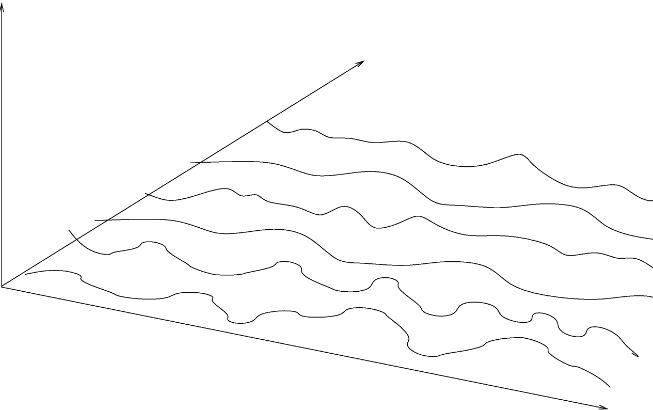
\includegraphics[scale=0.8]{day2_seg1_ranproc1/ensemble.jpg}
\end{frame}

\begin{frame}
  \onslide<1->{
	\frametitle{Random Processes} 
	\framesubtitle{Examples of Discrete Processes: Sampling with Replacement}
}
\begin{itemize}
  \onslide<2->{
			\item A card player shuffles a deck of cards and then picks a card at random.  
}
  \onslide<3->{
			\item He enters the value of the card (1 for an ace through 13 for a king) in an Excel spreadsheet column.  
}
  \onslide<4->{
			\item He then replaces the card and repeats the process over and over again.  
}
  \onslide<5->{
			\item After 10 such experiments, he begins anew with a new Excel column.  Each column represents a new sample trajectory. 
}
\end{itemize}
\end{frame}


\begin{frame}
  \onslide<1->{
	\frametitle{Random Processes} 
	\framesubtitle{Examples of Discrete Processes: MATLAB / Simulink Band-Limited White Noise}
}
\begin{itemize}
  \onslide<2->{
			\item A single source block (band-limited white noise) and a single sink (the scope).
}
  \onslide<3->{
			\item Each time the simulation is run, a new sample trajectory is generated.
}
  \onslide<4->{
			\item Note that this discrete process is created by supposedly sampling a continuous process.    
}
\end{itemize}
\end{frame}


\begin{frame}
  \onslide<1->{
	\frametitle{Random Processes} 
	\framesubtitle{Examples of Discrete Processes: MATLAB / Simulink Band-Limited White Noise}
}
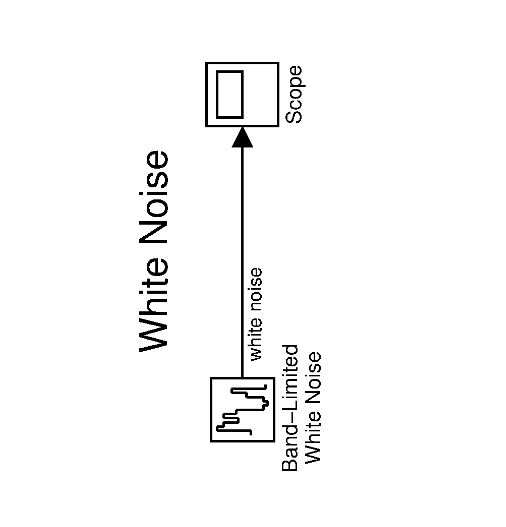
\includegraphics[angle=-90]{day2_seg1_ranproc1/white_noise.jpg}
\end{frame}


\begin{frame}
  \onslide<1->{
	\frametitle{Random Processes} 
	\framesubtitle{Examples:  MATLAB / Simunlink Random Constant}
}
\begin{itemize}
  \onslide<2->{
			\item A single source block (constant block with value generated by random number 
			generator) and a single sink (the scope).
}
  \onslide<3->{
			\item Each time the simulation is run, a new sample trajectory is generated.
}
  \onslide<4->{
			\item Note that this is a continuous process.  
}
\end{itemize}
\end{frame}

\begin{frame}
  \onslide<1->{
	\frametitle{Random Processes} 
	\framesubtitle{Examples:  MATLAB / Simunlink Random Constant}
}
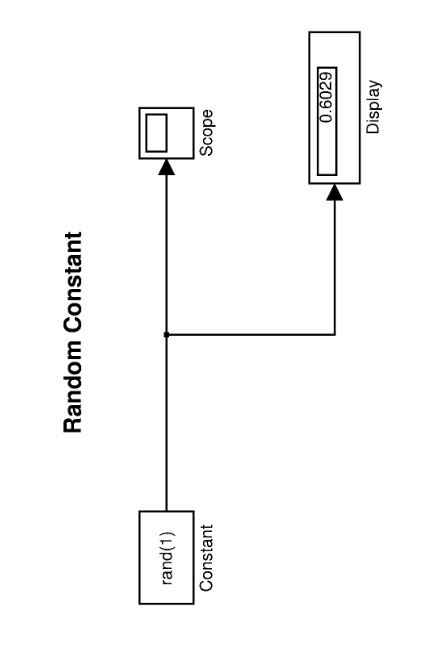
\includegraphics[angle=-90, scale=0.80]{day2_seg1_ranproc1/rand_const1.jpg}
\end{frame}


\begin{frame}
  \onslide<1->{
	\frametitle{Random Processes} 
	\framesubtitle{Examples:  MATLAB / Simunlink Random Constant}
}
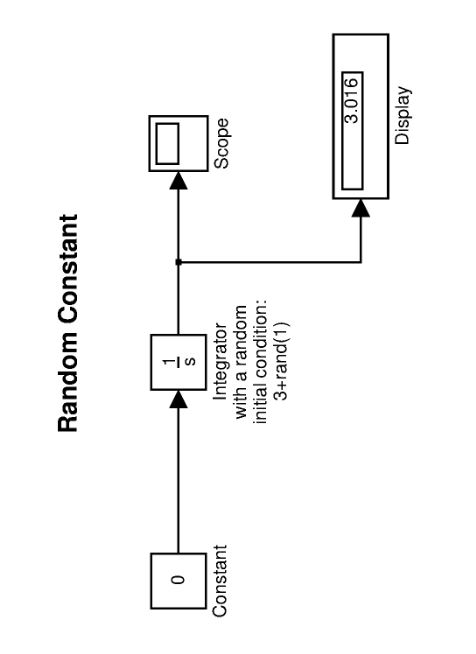
\includegraphics[angle=-90]{day2_seg1_ranproc1/rand_const2.jpg}
\end{frame}

\begin{frame}
  \onslide<1->{
	\frametitle{Random Processes} 
	\framesubtitle{MATLAB / Simulink Sine Wave with Random Phase}
}
\begin{itemize}
  \onslide<2->{
			\item A single source block (sine wave with random phase) and a single sink (the scope)
}
  \onslide<3->{
			\item Each time the simulation is run, a new sample trajectory is generated but 
			each time with a different value for the phase
}
  \onslide<4->{
			\item Note that this is a continuous process  
}
\end{itemize}
\end{frame}


\begin{frame}
  \onslide<1->{
	\frametitle{Random Processes} 
	\framesubtitle{MATLAB / Simulink Sine Wave with Random Phase}
}
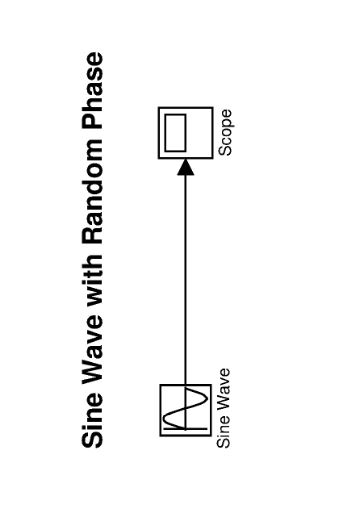
\includegraphics[angle=-90]{day2_seg1_ranproc1/sine_rand_phase.jpg}
\end{frame}
